\documentclass{VUMIFPSBakPrakAt}
\usepackage{float}
\usepackage{hyperref}
\usepackage{algorithmicx}
\usepackage{algorithm}
\usepackage{algpseudocode}
\usepackage{amsfonts}
\usepackage{amsmath}
\usepackage{bm}
\usepackage{caption}
\usepackage{color}
\usepackage{graphicx}
\usepackage{listings}
\usepackage{subcaption}
\usepackage{wrapfig}
\usepackage{biblatex}

% Titulinio aprašas
\university{Vilniaus universitetas}
\faculty{Matematikos ir informatikos fakultetas}
\department{Programų sistemų bakalauro studijų programa}
% Pavadinimo keisti nereikia - jis turi būti „Praktikos ataskaita“
\title{Praktikos ataskaita}
\author{Vardenis Pavardenis}
\status{Programų sistemų bakalauro 4 kursas}
\PracticeOrganization{UAB Pavyzdinė įmonė}
\OrganizationPracticeSupervisorRole{direktorius}
\OrganizationPracticeSupervisorName{Vardauskas Pavardauskas}
\UniversityPracticeSupervisor{prof. habil. dr. Vardaitis Pavardaitis}
\date{Vilnius, \the\year}

\bibliography{bibliografija}

\begin{document}
\maketitle

\tableofcontents

\sectionnonum{Įvadas}
Įvadas. Išdėstomi praktikos vietos pasirinkimo motyvai, praktikos užduotis, jos tikslas, spręstieji
uždaviniai, pateikiama praktinės veiklos planas praktikos atlikimo eiga (2--3 psl.).

\section{Įmonės / įstaigos apibūdinimas}
Įmonės/įstaigos apibūdinimas. Glaustai aprašoma įmonė/įstaiga, kurioje buvo atlikta praktika: jos
veiklos sritis, organizacinė struktūra, teikiamos paslaugos ir kt. Apibūdinamos praktikos vietoje
sudarytos darbo sąlygos (1--2 psl.).

Skyriai gali turėti poskyrius ir smulkesnes sudėtines dalis, kaip punktus ir
papunkčius.

\subsection{Poskyris}
Citavimo pavyzdžiai: cituojamas vienas šaltinis \cite{PvzStraipsnLt}; cituojami
keli šaltiniai \cite{PvzStraipsnEn, PvzKonfLt, PvzKonfEn, PvzKnygLt, PvzKnygEn,
PvzElPubLt, PvzElPubEn, PvzBakLt, PvzMagistrLt, PvzPhdEn}.

Anglų kalbos terminų pateikimo pavyzdžiai: priklausomybių injekcija (\anglnb{dependency injection},
dažnai trumpinama kaip \textit{DI}), saitų redaktorius \angl{linker}.

\subsection{Faktorialo algoritmas}

\ref{alg:factorial} pav. pateiktas faktorialo algoritmas.

\begin{algorithm}
\begin{algorithmic}[1] % [1] padaro, kad eilutės būtų sunumeruotos
\State $N\gets$ skaičius, kurio faktorialą skaičiuojame
\State $F\gets 1$
\For{$i := 2$ $to$ $N$}
    \State $F\gets F \cdot i$
\EndFor
\end{algorithmic}
\caption{Faktorialo algoritmas}
\label{alg:factorial}
\end{algorithm}

\subsubsection{Punktas}
\subsubsubsection{Papunktis}
\subsubsection{Punktas}

\section{Praktikos veiklos aprašymas}
Praktikos veiklos aprašymas (vienas arba keli skyriai). Aprašomas praktikos užduoties
įgyvendinimas (pvz., atlikti projektavimo ir/ar programavimo darbai, sukurtas modelis, priimti
sprendimai ir pan.).

\subsection{Poskyris}
\subsection{Poskyris}

\sectionnonum{Rezultatai, išvados ir pasiūlymai}
Rezultatai, išvados ir pasiūlymai. Išdėstomi pagrindiniai darbo rezultatai ir išvados, praktikos
darbo privalumai ir trūkumai, aprašomos įgytos žinios ir patirtis praktikos metu, duodamas
universitete įgytų žinių atitikimo praktikos užduočiai atlikti įvertinimas, pateikiami argumentuoti
pasiūlymai, kaip geriau organizuoti darbo ir valdymo procesus praktikos atlikimo vietoje ir
mokymą Universitete (1--2 psl.).

% Bibliografija (jeigu yra ką ten dėti)
\printbibliography[heading=bibintoc]

% Sąvokų apibrėžimai ir santrumpų sąrašas sudaromas tada, kai darbo tekste
% vartojami specialūs paaiškinimo reikalaujantys terminai ir rečiau sutinkamos
% santrumpos.
%\sectionnonum{Sąvokų apibrėžimai}
%\sectionnonum{Santrumpos}

% Priedai. Pateikiama pagalbinė medžiaga: didelės schemos, lentelės, paveiksliukai,
% kurie reikalingi pateikiamam darbui aprašyti ir pristatyti.
\appendix{Neuroninio tinklo struktūra}
\begin{figure}[H]
    \centering
    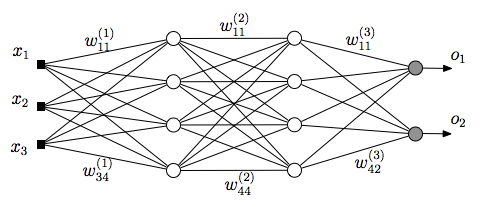
\includegraphics[scale=0.5]{img/MLP}
    \caption{Paveikslėlio pavyzdys}
    \label{img:mlp}
\end{figure}


\appendix{Eksperimentinio palyginimo rezultatai}
% tablesgenerator.com - converts calculators (e.g. excel) tables to LaTeX
\begin{table}[H]\footnotesize
  \centering
  \caption{Lentelės pavyzdys}
  {\begin{tabular}{|l|c|c|} \hline
    Algoritmas & $\bar{x}$ & $\sigma^{2}$ \\
    \hline
    Algoritmas A  & 1.6335    & 0.5584       \\
    Algoritmas B  & 1.7395    & 0.5647       \\
    \hline
  \end{tabular}}
  \label{tab:table example}
\end{table}

\end{document}
